% ex: ts=2 sw=2 sts=2 et filetype=tex
% SPDX-License-Identifier: CC-BY-SA-4.0

\documentclass[12pt,addpoints]{exam}

\usepackage[utf8]{inputenc}
\usepackage[T1]{fontenc}
%\usepackage[spanish]{babel}
\usepackage[letterpaper]{geometry}
\usepackage{pgfplots}

\pagestyle{headandfoot}
\headrule
\header{Geometría Analítica}{Examen}{CBTIS 246}
\footer{}{Página \thepage\ de \numpages}{}

\pointpoints{punto}{puntos}
\renewcommand{\solutiontitle}{\textbf{Solución: }}

\printanswers

\begin{document}
\begin{center}
\fbox{\fbox{\parbox{5.5in}{\centering
Lee con atención cada pregunta y responde en
el espacio ubicado en la parte izquierda.
}}}
\end{center}

\vspace{5mm}

Nombre:\enspace\hrulefill

\vspace{5mm}

Grupo:\enspace\hrulefill
\enspace{}Grado:\enspace\hrulefill
\enspace{}Fecha:\enspace\hrulefill

\begin{questions}

% ex: ts=2 sw=2 sts=2 et filetype=tex
% SPDX-License-Identifier: CC-BY-SA-4.0

\question Las moléculas de los \fillin\ se pueden mover libremente debido a
  que la fuerza de atracción son más débil que en los sólidos, lo que permite
  que tengan mayor libertad de rotación y traslación, además de la vibración.

  \begin{oneparchoices}
    \CorrectChoice Líquidos
    \choice Plasma
    \choice Gaseosos
    \choice Sólidos
  \end{oneparchoices}
  \answerline[A]

% ex: ts=2 sw=2 sts=2 et filetype=tex
% SPDX-License-Identifier: CC-BY-SA-4.0

\question Los \fillin\ se caracterizan porque las partículas que
los componen están muy cercanas entre sí, y en posiciones más o menos fijas

  \begin{oneparchoices}
    \choice Líquidos
    \CorrectChoice Sólidos
    \choice Gaseosos
    \choice Todos
  \end{oneparchoices}
  \answerline[B]

% ex: ts=2 sw=2 sts=2 et filetype=tex
% SPDX-License-Identifier: CC-BY-SA-4.0

\question Es el lado opuesto al ángulo recto en un triángulo rectángulo.

  \begin{oneparchoices}
    \CorrectChoice Hipotenusa
    \choice $c^2 = a^2 + b^2$
    \choice Cateto
    \choice Lado recto
  \end{oneparchoices}
  \answerline[A]

\input{p/p01t3}
\clearpage
% ex: ts=2 sw=2 sts=2 et filetype=tex
% SPDX-License-Identifier: CC-BY-SA-4.0

\question Usa la siguiente cuadricula para resolver los siguientes incisos:

  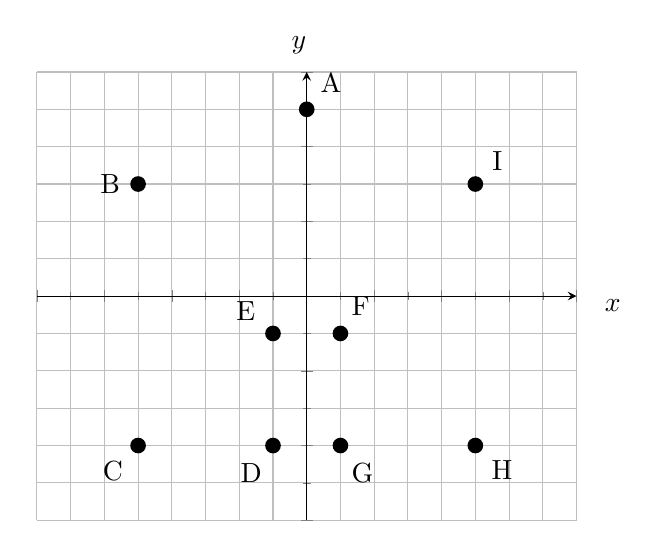
\begin{tikzpicture}
    \begin{axis}[grid=both,ymin=-6,ymax=6,xmax=8,xmin=-8,xticklabel=\empty,yticklabel=\empty,
               minor tick num=1,axis lines = middle,xlabel=$x$,ylabel=$y$,
               label style = {at={(ticklabel cs:1.1)}}]
      \node[label={60:{A}},circle,fill,inner sep=2pt] at (axis cs:0,5) {};
      \node[label={180:{B}},circle,fill,inner sep=2pt] at (axis cs:-5,3) {};
      \node[label={30:{I}},circle,fill,inner sep=2pt] at (axis cs:5,3) {};
      \node[label={230:{C}},circle,fill,inner sep=2pt] at (axis cs:-5,-4) {};
      \node[label={320:{H}},circle,fill,inner sep=2pt] at (axis cs:5,-4) {};
      \node[label={160:{E}},circle,fill,inner sep=2pt] at (axis cs:-1,-1) {};
      \node[label={80:{F}},circle,fill,inner sep=2pt] at (axis cs:1,-1) {};
      \node[label={260:{D}},circle,fill,inner sep=2pt] at (axis cs:-1,-4) {};
      \node[label={280:{G}},circle,fill,inner sep=2pt] at (axis cs:1,-4) {};
    \end{axis}
  \end{tikzpicture}

  \begin{parts}
    \part Encuantra las coordenadas de los vértices en el polígono. \\
    A(\fillin\ ,\fillin\ ) \enspace B(\fillin\ ,\fillin\ ) \\
    C(\fillin\ ,\fillin\ ) \enspace D(\fillin\ ,\fillin\ ) \\
    E(\fillin\ ,\fillin\ ) \enspace F(\fillin\ ,\fillin\ ) \\
    G(\fillin\ ,\fillin\ ) \enspace H(\fillin\ ,\fillin\ ) \\
    I(\fillin\ ,\fillin\ ) \\
    \part Determina el cuadrante en el que se ubica los puntos: \\
    El punto B esta en el cuadrante:\fillin \\
    El punto C esta en el cuadrante:\fillin \\
    El punto D esta en el cuadrante:\fillin \\
    El punto E esta en el cuadrante:\fillin \\
    El punto F esta en el cuadrante:\fillin \\
    El punto G esta en el cuadrante:\fillin \\
    El punto H esta en el cuadrante:\fillin \\
    El punto I esta en el cuadrante:\fillin \\
    \part Sacar la distancia entre los puntos: \\
    AB \fillin \enspace BC \fillin \enspace CD \fillin \enspace DE \fillin \enspace \\
    EF \fillin \enspace FG \fillin \enspace GH \fillin \enspace HI \fillin \enspace  \\
    IA \fillin \enspace
    \part Calcula el perímetro de la figura resultante.
  \end{parts}


\end{questions}

\end{document}
